%%
% This is an Overleaf template for scientific articles and reports
% using the TUM Corporate Desing https://www.tum.de/cd
%
% For further details on how to use the template, take a look at our
% GitLab repository and browse through our test documents
% https://gitlab.lrz.de/latex4ei/tum-templates.
%
% The tumarticle class is based on the KOMA-Script class scrartcl.
% If you need further customization please consult the KOMA-Script guide
% https://ctan.org/pkg/koma-script.
% Additional class options are passed down to the base class.
%
% If you encounter any bugs or undesired behaviour, please raise an issue
% in our GitLab repository
% https://gitlab.lrz.de/latex4ei/tum-templates/issues
% and provide a description and minimal working example of your problem.
%%


\documentclass[
  english,        % define the document language (english, german)
  font=times,     % define main text font (helvet, times, palatino, libertine)
  twocolumn,      % use onecolumn or twocolumn layout
]{tumarticle}


% load additional packages
\usepackage{lipsum}
\usepackage{svg}
\usepackage{wrapfig}
\usepackage{amsmath}
\usepackage[nameinlink]{cleveref}
\usepackage[style=numeric]{biblatex}
\usepackage{csquotes}
\usepackage{booktabs}
\usepackage{tabularx}
\usepackage{stfloats}
\addbibresource{refs.bib}

% article metadata
\title{Reducing Training Resource Cost by Selective Parameter Updating}

\author[affil=1, email=baykam.say@tum.de]{Baykam Say}
\author[affil=1, email=baris.coslu@tum.de]{Coşku Barış Coşlu}
\author[affil=1, email=mato.gudelj@tum.de]{Mato Gudelj}

\affil[mark=1]{\theDepartmentName, \theUniversityName}

\date{June 24, 2023}


\begin{document}

\maketitle

\begin{abstract}
  This work introduces two novel Parameter-Efficient Fine Tuning (PEFT) methods for fine-tuning of large-scale pre-trained transformer models, Singular Value Adaptation (SiVA) and k-Ladder Side-Tuning (k-LST). Additionally, it utilizes input prompts to improve the performance of PEFT methods. SiVA improves upon LoRA by leveraging singular value decomposition for initialization, thereby avoiding the problematic zero-initialization employed by LoRA. This leads to faster convergence while maintaining full fine-tuning performance. k-LST improves upon Ladder Side Tuning, closing the performance gap of memory efficient PEFT methods while retaining a low memory footprint. It extracts backbone features with a sliding window, which are then queried by the side network with cross-attention. Prompts, when used in conjunction with various PEFT methods, improve performance over the baseline with no computational drawbacks.
\end{abstract}

\section{Introduction}

In recent  years, large-scale pre-training and fine-tuning of transformer models have been prominent in domains such as natural language processing (NLP), computer vision (CV), and vision-and-language (VL) tasks. These models have the capacity to learn a wide spectrum of features from extensive data, making them highly effective for a variety of tasks. However, as the size of these models increases, the computational expense for fine-tuning becomes substantial

In an effort to mitigate this issue, Parameter-Efficient Fine Tuning (PEFT) has become a notable area of research. The objective of PEFT is to build models that can proficiently handle multiple tasks without the need to train an entirely new model for each task. This is accomplished by updating a small subset of pre-trained parameters or by incorporating new additional parameters into the pre-trained network, while the majority of the original parameters remain unchanged. The focus of PEFT is to efficiently adapt pre-trained models to new tasks by reducing the overhead of fine-tuning.

In general, PEFT methods have a trade-off between model performance, memory efficiency, and fine-tuning speed. This inherent trade-off between model efficiency and performance is a challenge that needs to be addressed to fully harness the potential of PEFT techniques in resource-constrained environments. This work is focused on addressing this trade-off by proposing novel methods that seek to balance efficiency and performance during PEFT.

PEFT methods can be categorized by their underlying approach to achieving parameter efficiency. We use the three-class taxonomy that divides PEFT methods into additive, selective, and reparametrization-based methods \cite{peft-categories}:

Additive methods insert extra parameters or layers into the pre-trained model and only train these newly inserted parameters. Well-known examples include Adapters \cite{adapters} and prompt tuning \cite{prompt-tuning}. Adapters are compact modules inserted into transformer blocks, while prompt tuning uses a small set of parameters that are concatenated with input embeddings. A recent addition to this category is LST \cite{sung2022lst}, which trains a small side model that operates on intermediate features of the original model, which are passed laterally to it. This is particularly memory efficient. 

Selective methods keep the original model and update a subset of the parameters instead of all. BitFit \cite{zaken2022bitfit} is one example of such a method. BitFit only updates the bias parameters (or a small subset of them) to fine-tune the model.

Reparametrization-based methods leverage low-rank representations of the weights to update smaller matrices that reflect the whole model. LoRA \cite{hu2021lora} is the most common example, and it trains low-rank matrices that represent the change in the full-rank weight matrices.

Our work covers two of the given categories: reparametrization-based methods and additive methods (extending LST). We focus on reparametrization-based methods since they are relatively new and widely used in the industry and we focus on LST since it is a state-of-the-art additive method that uses minimal memory. We also work on improving PEFT methods through external factors. These include pre-fine-tuning the original model before PEFT using MeZO \cite{mezo}, a recent low-memory optimizer for PEFT, and modifying the model prompts for PEFT.

\section{Related Work}
\subsection{Reparametrization-based Methods}
Research has shown that the intrinsic dimensions of a model reduce when it is fine-tuned for a specific task \cite{aghajanyan2020intrinsic}. Therefore, in theory, a low-dimension reparametrization that is as effective as the full parameter space can be used for fine-tuning \cite{aghajanyan2020intrinsic}.

\subsubsection{LoRA}
LoRA \cite{hu2021lora} uses this information and the hypothesis that the updates made during fine-tuning also have a low intrinsic dimension to create a low-rank weight updating PEFT method. It works on the weight matrices of linear layers by inserting two trainable lower-rank matrices (LoRA weights) that represent the change of the original matrix as seen on \Cref{lora-reparam}.

\begin{figure}[h]
    \centering
    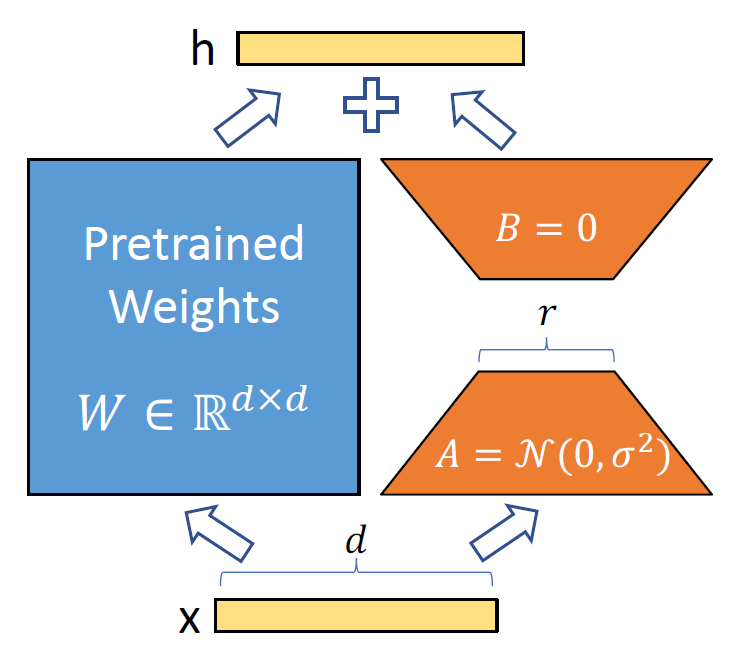
\includegraphics[width=0.6\linewidth]{assets/images/lora-reparametrization.png}
    \caption{The reparametrization of LoRA \cite{hu2021lora}. Only A and B are trained.}
    \label{lora-reparam}
\end{figure}

During training, the pretrained weight matrix (\(W_0\)) of the linear layer is frozen, and the LoRA weights, represented by a down projection (\(A\)) and an up projection (\(B\)) layer, are trained. During the forward pass, the two lower-rank matrices are multiplied together and then added to the original matrix to generate the updated weight matrix for that specific linear layer. For a linear transformation \(h = W_0 x\), the modified forward pass of LoRA yields:

\begin{equation}
    h = W_0 x + B A x
\end{equation}

The down projection layer is randomly initialized, while the up projection layer is initialized to zero. This ensures that their initial multiplication, which represents the change of the weight matrix, is zero. For inference, LoRA weights can be merged with the original weight matrix to get an unmodified model that has the updated weight matrices.

\subsubsection{LoRA-like Models}
Recent advancements in reparametrization-based methods have all used the same approach of freezing the original weight matrix and representing the updates on lower-rank update matrices. These methods include KronA \cite{edalati2022krona}, which uses the Kronecker products of two low-rank matrices to represent the updates; IA\textsuperscript{3} \cite{ia3}, which reimplements the forward pass of LoRA as \(h = (W_0 (x \circ A)) \circ B\) and applies LoRA to only the key and value layers in self-attention and the feed-forward layers in the transformer; and QLoRA \cite{dettmers2023qlora}, which keeps the original weights in a lower-precision data type while applying LoRA. We compare our method directly to LoRA as the other reparametrization-based methods use the same approach and only introduce incremental improvements over LoRA.
\subsection{LST}
Ladder Side-Tuning (LST) \cite{sung2022lst} is a recent advancement in the area of memory-efficient PEFT that has a significantly smaller memory footprint compared to other methods. The method achieves memory efficiency by circumventing the need to backpropagate through the large pre-trained backbone. Unlike other techniques that incorporate parameters into the pre-trained backbone network, LST involves training a small, separate ladder side network. This side network takes intermediate activations from the backbone network via lateral side connections (Shown in \Cref{lst-original}).

While LST represents a significant advancement in terms of memory efficiency during training, its observed performance is lower compared to other state-of-the-art (SOTA) PEFT techniques. The design of LST, which prevents the method from directly affecting the backbone's forward pass, appears to limit its ability to fully leverage the pre-training of the original model.

\begin{figure}[h]
    \centering
    %\includegraphics[width=0.7\linewidth]{assets/images/LST.png}
    \includesvg[width=0.65\linewidth]{assets/images/LST.svg}
    \caption{The original LST architecture for an encoder-only backbone. The intermediate backbone representations are downsampled to a dimension of \(d/r\), after which they are fused with the side network features. The gradients of the trainable parameters (shown in green) are computed without going through the backbone network (shown in blue).}
    \label{lst-original}
\end{figure}
\subsection{MeZO}
Zeroth-order optimization (ZO-SGD \cite{zo-sgd}) estimates gradients using only forward-passes, making it possible to update neural networks without backpropagation. Memory-efficient Zeroth-order Optimizer (MeZO \cite{mezo})  is an adaptation of the classical zeroth-order optimization method, reducing its memory consumption by operating in-place. This results in a method that is able to fine-tune LMs with the same memory footprint as inference. 
%The authors prove that MeZO can successfully optimize LLMs and show its efficiency 

To estimate gradients, MeZO uses Simultaneous Perturbation Stochastic Approximation (SPSA), which requires two forward passes to estimate the gradient. For each forward pass, the parameters of the model are perturbed by different amounts, depending on a random number sampled for each parameter and the perturbation scale, which is a hyperparameter of the model. For loss function $\mathcal{L}$, model parameters $\mathbf{\theta} \in \mathbb{R}^d$ and minibatch $\mathcal{B}$, SPSA estimates gradient as:

\begin{equation}
    \hat{\nabla}\mathcal{L}(\mathbf{\theta}; \mathcal{B}) = 
    \frac{\mathcal{L}(\mathbf{\theta} + \epsilon\mathbf{z}; \mathcal{B}) - \mathcal{L}(\mathbf{\theta} - \epsilon\mathbf{z}; \mathcal{B})}
    {2 \epsilon} \mathbf{z}
\end{equation}

where $\epsilon$ is the perturbation scale and $\mathbf{z} \in \mathbb{R}^d$ is randomly sampled with $\mathbf{z} \sim \mathcal{N}(0, \textbf{\em I}_d)$. 

Using the SPSA estimate for gradients, the model is updated with SGD:

\begin{equation}
    \mathbf{\theta}_{t+1} = \mathbf{\theta}_t - \eta \hat{\nabla} \mathcal{L}(\mathbf{\theta}; \mathcal{B}_t)
\end{equation}

where $\eta$ is the learning rate. 

MeZO's in-place implementation saves additional memory for this approach. For each batch, MeZO samples a random seed and every time a parameter gets updated or perturbed for the gradient estimation, it samples the random value \textbf{z} using this seed. This way, $\mathbf{z} \in \mathbb{R}^d$ does not need to be stored, theoretically reducing memory consumption to the same as inference. In practice, often entire weight matrices are perturbed instead of individual scalars, saving time but costing additional memory as large as the largest weight matrix. 

\subsubsection{Prompt-based Fine-tuning}

Experiments show that prompting is crucial for the ability of MeZO to optimize the network. Thus, MeZO is used under the prompt-based fine-tuning setting described in \cite{prompt}. 

For each example in the dataset, a model is given a prompt as input; this prompt is a template attached to the input sentence and varies depending on the task and dataset. The template contains a mask token and the model is trained to predict the masked word from a set of label words, where each label word is assigned to one label. Classification is then performed using the logits of the label words on the mask token. \Cref{fig:prompt} shows how prompt-based fine-tuning works on the SST-2 dataset. 

\begin{figure}
    \centering
    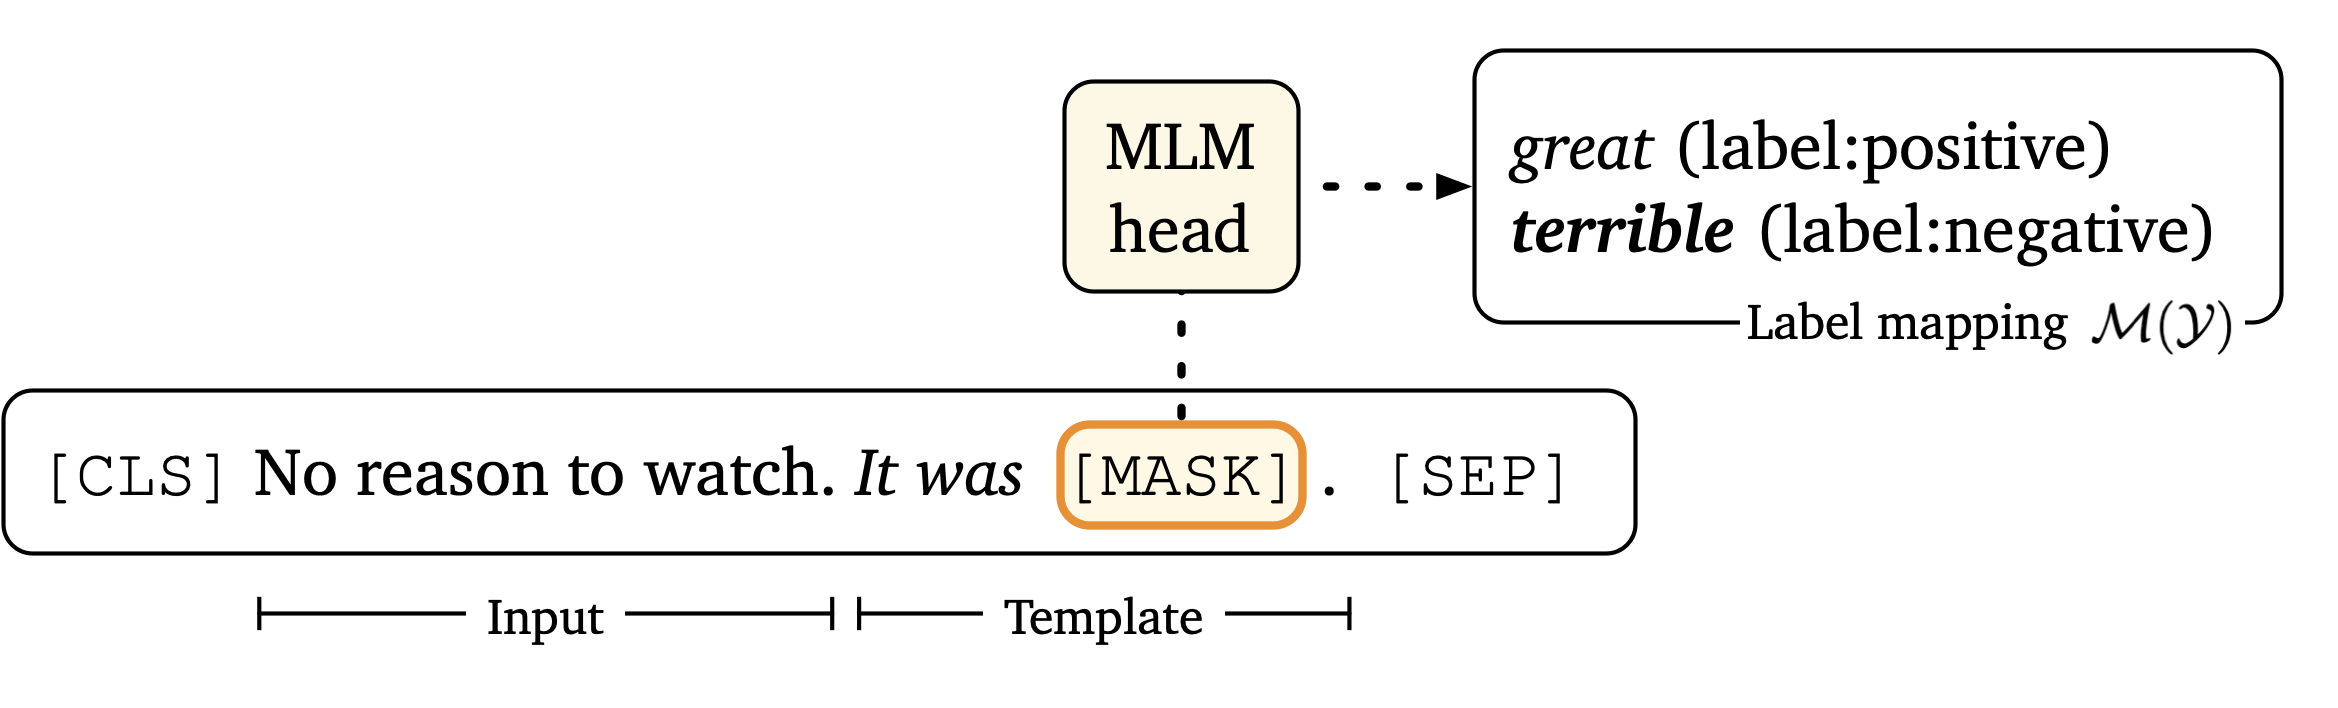
\includegraphics[width=\linewidth]{assets/images/Prompt.png}
    \caption{Prompt-based fine-tuning on SST-2. Adapted from \cite{prompt}. The prompt consists of the input sentence and the template \textit{"It was [MASK]."}. The model is trained to predict the label word \textit{"great"} for positive input sentences and \textit{"terrible"} for negative input sentences.}
    \label{fig:prompt}
\end{figure}

\section{Methods}
This section is split into three subsections, each explaining a separate approach to improve parameter efficient fine-tuning.
\subsection{Singular Value Adaptation (SiVA)}

During our research, we focused on the main weakness of LoRA-like models: using random and zero initializations for their layers. While this allows them to initially represent the weight updates as zero, it also harms the training as the optimizer struggles with zero initialization. As a solution, we propose a novel low-rank fine-tuning method: Singular Value Adaptation (SiVA). SiVA represents the whole weight matrix in a lower rank using singular value decomposition instead of representing just the change in the weights like LoRA. 

\subsubsection{Model Initialization}
The initialization of SiVA is shown in \Cref{siva-init}. To accomplish this, it first decomposes the original weight matrix \(W_0\) into \(U, S, V\) matrices using SVD, where S is a one-dimensional matrix consisting of the diagonal elements of the rectangular diagonal matrix \(\Sigma\) and \(V = V_0^H\):

\begin{equation}
    W_0 = U \Sigma V_0^H
\end{equation}

It then splits \(U, S, V\) matrices into training and reconstruction matrices. Training (\(U_t, S_t, V_t\)) matrices are rank \(r\) matrices where \(r\) represents the rank of the training and they contain the highest singular value row and columns:

\begin{align}
    U_t &= U[:, [1, 2, ..., r]]\\
    S_t &= S[1, 2, ..., r]\\
    V_t &= V[[1, 2, ..., r],:]
\end{align}

Reconstruction (\(U_r, S_r, V_r\)) matrices are rank \(d-r\) matrices where \(d\) is the decomposition rank and they contain the remaining rows and columns until \(d\). \(d\) is a hyperparameter to allow lossy reconstruction of the weight matrix to reduce overfitting of the initial model similar to pruning with SVD.

\begin{align}
    U_r &= U[:, [r, r+1, ..., d]]\\
    S_r &= S[r, r+1, ..., d]\\
    V_r &= V[[r, r+1, ..., d],:]
\end{align}

The original matrix is then reconstructed using the reconstruction matrices and frozen. The resulting matrix \(W_r\) denotes the lost granularity of the low-rank representation:

\begin{equation}
    W_r = U_r \circ S_r V_r
\end{equation}

Only \(U_t\) and \(V_t\) matrices are trained. Since they are the most impactful parts of the original weight matrix according to singular value decomposition, their updates represent the updates over the original weight matrix as accurately as possible. 

\begin{figure}[t]
    \centering
    \includesvg[width=0.75\linewidth]{assets/images/siva-init}
    \caption{SiVA initialization diagram. The original weight matrix \(W_0\) is decomposed using SVD. Rank \(r\) submatrices of the decomposition are selected according to the highest singular values (\(U_t, S_t, V_t\)). Original matrix is reconstructed without including (\(U_t, S_t, V_t\)). Only \(U_t, V_t\) are trained. }
    \label{siva-init}
\end{figure}

\begin{figure*}[htb]
    \centering
    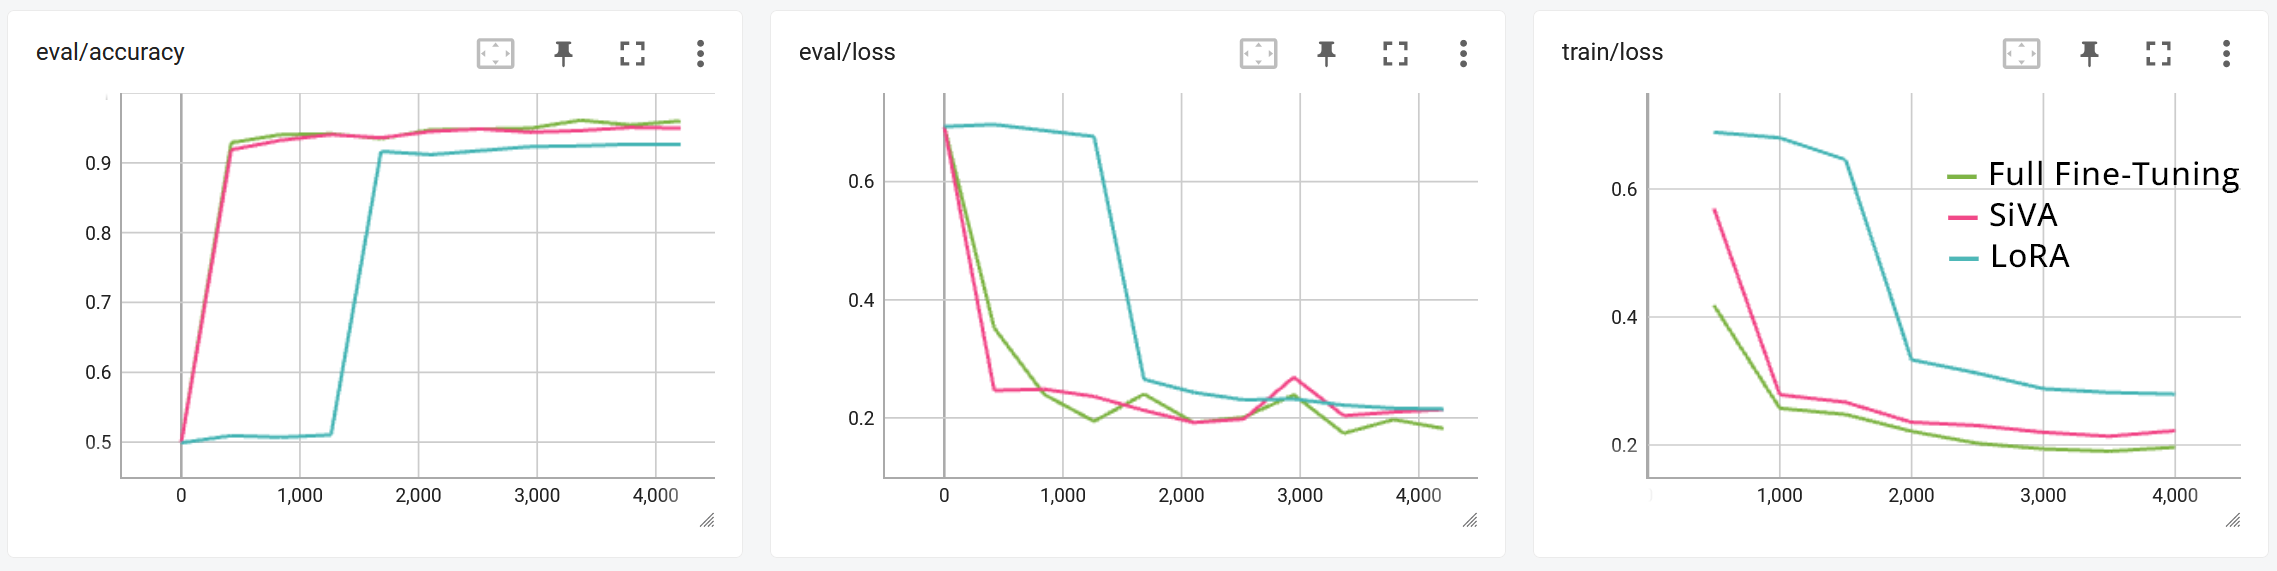
\includegraphics[width=\textwidth]{assets/images/siva-lora-training.png}
    \caption{The training graphs for full fine-tuning, SiVA, and LoRA for RoBERTa-large \cite{roberta} on the SST-2 \cite{wang2019glue} dataset for one epoch. Full fine-tuning and SiVA follow each other closely in all graphs while LoRA has worse performance. All the hyperparameters are the same, the original model initialization (including the head) is also the same. No smoothing applied.}
    \label{siva-lora-training}
\end{figure*}

\subsubsection{Forward Pass}
During the forward pass, training matrices are reconstructed and added to \(W_r\) to get the updated weight matrix without any loss of granularity from the lower-rank representation. For \(h = W_0 x\), the modified forward pass yields:

\begin{equation}
    h = W_r x + U_t \circ S_t V_t x
\end{equation}

\begin{figure}[htb]
    \centering
    \includesvg[width=\linewidth]{assets/images/lora-siva-forward-pass}
    \caption{Visual representation of the forward passes of LoRA and SiVA. In both figures, the trainable parts (\(A, B\) for LoRA and \(U_t, V_t\) for SiVA) are multiplied and added to the untrainable part to get the updated weight matrix. A linear transformation is applied with the resulting updated matrix to get the results. LoRA's trainable parts represent the change in the original matrix while SiVA's trainable parts represent the whole matrix.}
    \label{lora-siva}
\end{figure}

\Cref{lora-siva} shows the comparison between LoRA's and SiVA's forward passes. Recall that the modified forward pass of LoRA is formulized as \(h = W_0 x + B A x\). While \(A, B\) are same size matrices as \(U_t, V_t\); \(A, B\) represent only the change of the original matrix whereas \(U_t, V_t\) represent the whole matrix. 

\subsubsection{Optimal Hyperparameters}
SiVA introduces two new hyperparameters. For the training rank, we use \(r=4\) to reach the full fine-tuning performance on RoBERTa-large. We hypothesize that as the model size grows, \(r\) can get as low as \(1\) without losing any performance similar to LoRA. We use the number of output channels of \(W_0\) for the decomposition rank \(d\). Selecting a lower \(d\) reduces accuracy. Moreover, we experiment with training a subset of linear layers with SiVA and freezing the rest. We find the best balance between accuracy and efficiency when training only the key and query projection matrices in self attention.

\subsubsection{Comparing to LoRA and Full Fine-Tuning}
Similar to LoRA, training matrices of SiVA can be merged after training to get an unmodified model to remove any inference latency. They can also be swapped with other training matrices to modify the same base model for different fine-tuned tasks, eliminating the need for keeping multiple fine-tuned large models for different tasks. However, unlike LoRA, since SiVA does not have zero or random initialization, the optimization is easier and the training converges much faster.

As it can be seen from \Cref{siva-lora-training}, the training graphs of full fine-tuning and SiVA are almost identical, to the fluctuations of the unsmoothed graphs, whereas LoRA struggles to have any meaningful optimizations in the first quarter of the epoch due to the random and zero initializations of its layers. Even if we shift the LoRA graph left 1000 iterations to mitigate 50\% accuracy of the first quarter, we can observe that the accuracy and loss are still worse compared to full fine-tuning and SiVA. Due to the similarity of the training graphs of SiVA and full fine-tuning with the same hyperparameters, we claim that SiVA is analogous to full fine-tuning in a lower dimension.

\subsection{k-Ladder Side-Tuning (k-LST)}

In an attempt to close the performance gap for memory efficient PEFT, we introduce k-Ladder Side-Tuning (k-LST). This is a generalization of Ladder Side-Tuning (LST) \cite{sung2022lst}, where LST can be considered a special case of our generalized method for \(k = 1\). Each block of the LST side network takes the corresponding intermediate activation from the backbone as a side input. The k-LST extends this approach by taking a sliding window of $k$ backbone features, as well as employing a more intricate fusion approach through cross attention. We demonstrate that the proposed method significantly closes the performance gap to other PEFT methods while retaining a low memory footprint.


\subsubsection{Sliding k-window}
The k-LST method employs backbone features extracted from a \(k\) sized sliding window (see \Cref{fig:k-LST}). The window for the \(i\)-th side feature is centered at the \(i\)-th backbone block. For cases when the window overflows we employ padding with zeros. As in \cite{sung2022lst}, we downsample each of these features to dimension \(\frac{d}{r}\), where \(r\) is the reduction factor hyperparameter. This is done with a learned linear projection:

\begin{equation}
C_i = d_j(B_j),
\end{equation}

where $C_i$ is the $i$-th feature in the window. The weights of the linear projections are \textit{not} shared.

\subsubsection{Feature Fusion With Cross Attention}
These downsampled features are queried using a cross attention mechanism. During training, we use random dropout \cite{JMLR:v15:srivastava14a} with a probability of \(p\) and add a trainable positional encoding \(\vec{p_i}\) to encode the window location of each feature:

\begin{equation}
    \tilde{C_i} = \text{{Dropout}}(C_i, \text{{is\_training}}) + \vec{p_i}.
\end{equation}

To construct the final matrix, we concatenate the features \(\tilde{C_i}\) without adding a new axis:
\begin{equation}
C_{j-w:j+w} = \begin{bmatrix} \tilde{C_1} \\ \tilde{C_2} \\ \vdots \\ \tilde{C_k} \end{bmatrix},
\end{equation}

where \(j\) is the index of the center block and

\begin{equation}
    w = \left\lfloor{\frac{k}{2}}\right\rfloor.
\end{equation}

For the cross attention operation, we derive the query vectors (\(Q\)) from the \(j-1\)-th layer of the trainable side network, symbolized as \(\theta_{j-1}\). The key and value vectors (\(K\) and \(V\)) are obtained from the concatenated features \(C_{j-w:j+w}\)

\begin{align}
    &Q_j = \theta_{j-1} \\
    &K_j = V_j = C_{j-w:j+w}.
\end{align}

The output of the \(j\)-th layer of the side network \(\theta_j\) is then computed using the cross attention mechanism, followed by the side block: 
\begin{align}
X_j &= \text{{CrossAttention}}(Q_jW^q, K_jW^k, V_jW^v) \\
\theta_j &= \text{{SideBlock}}_j(X_j)
\end{align}

The side block is a simple transformer encoder block, mirroring the architecture of the backbone. If \(\theta_j\) is the output of the last block before the output, we upsample the feature with a linear up-projection and pass it to the classification head (Illustrated in \Cref{fig:k-LST}).


\begin{figure*}[htb]
    \centering
    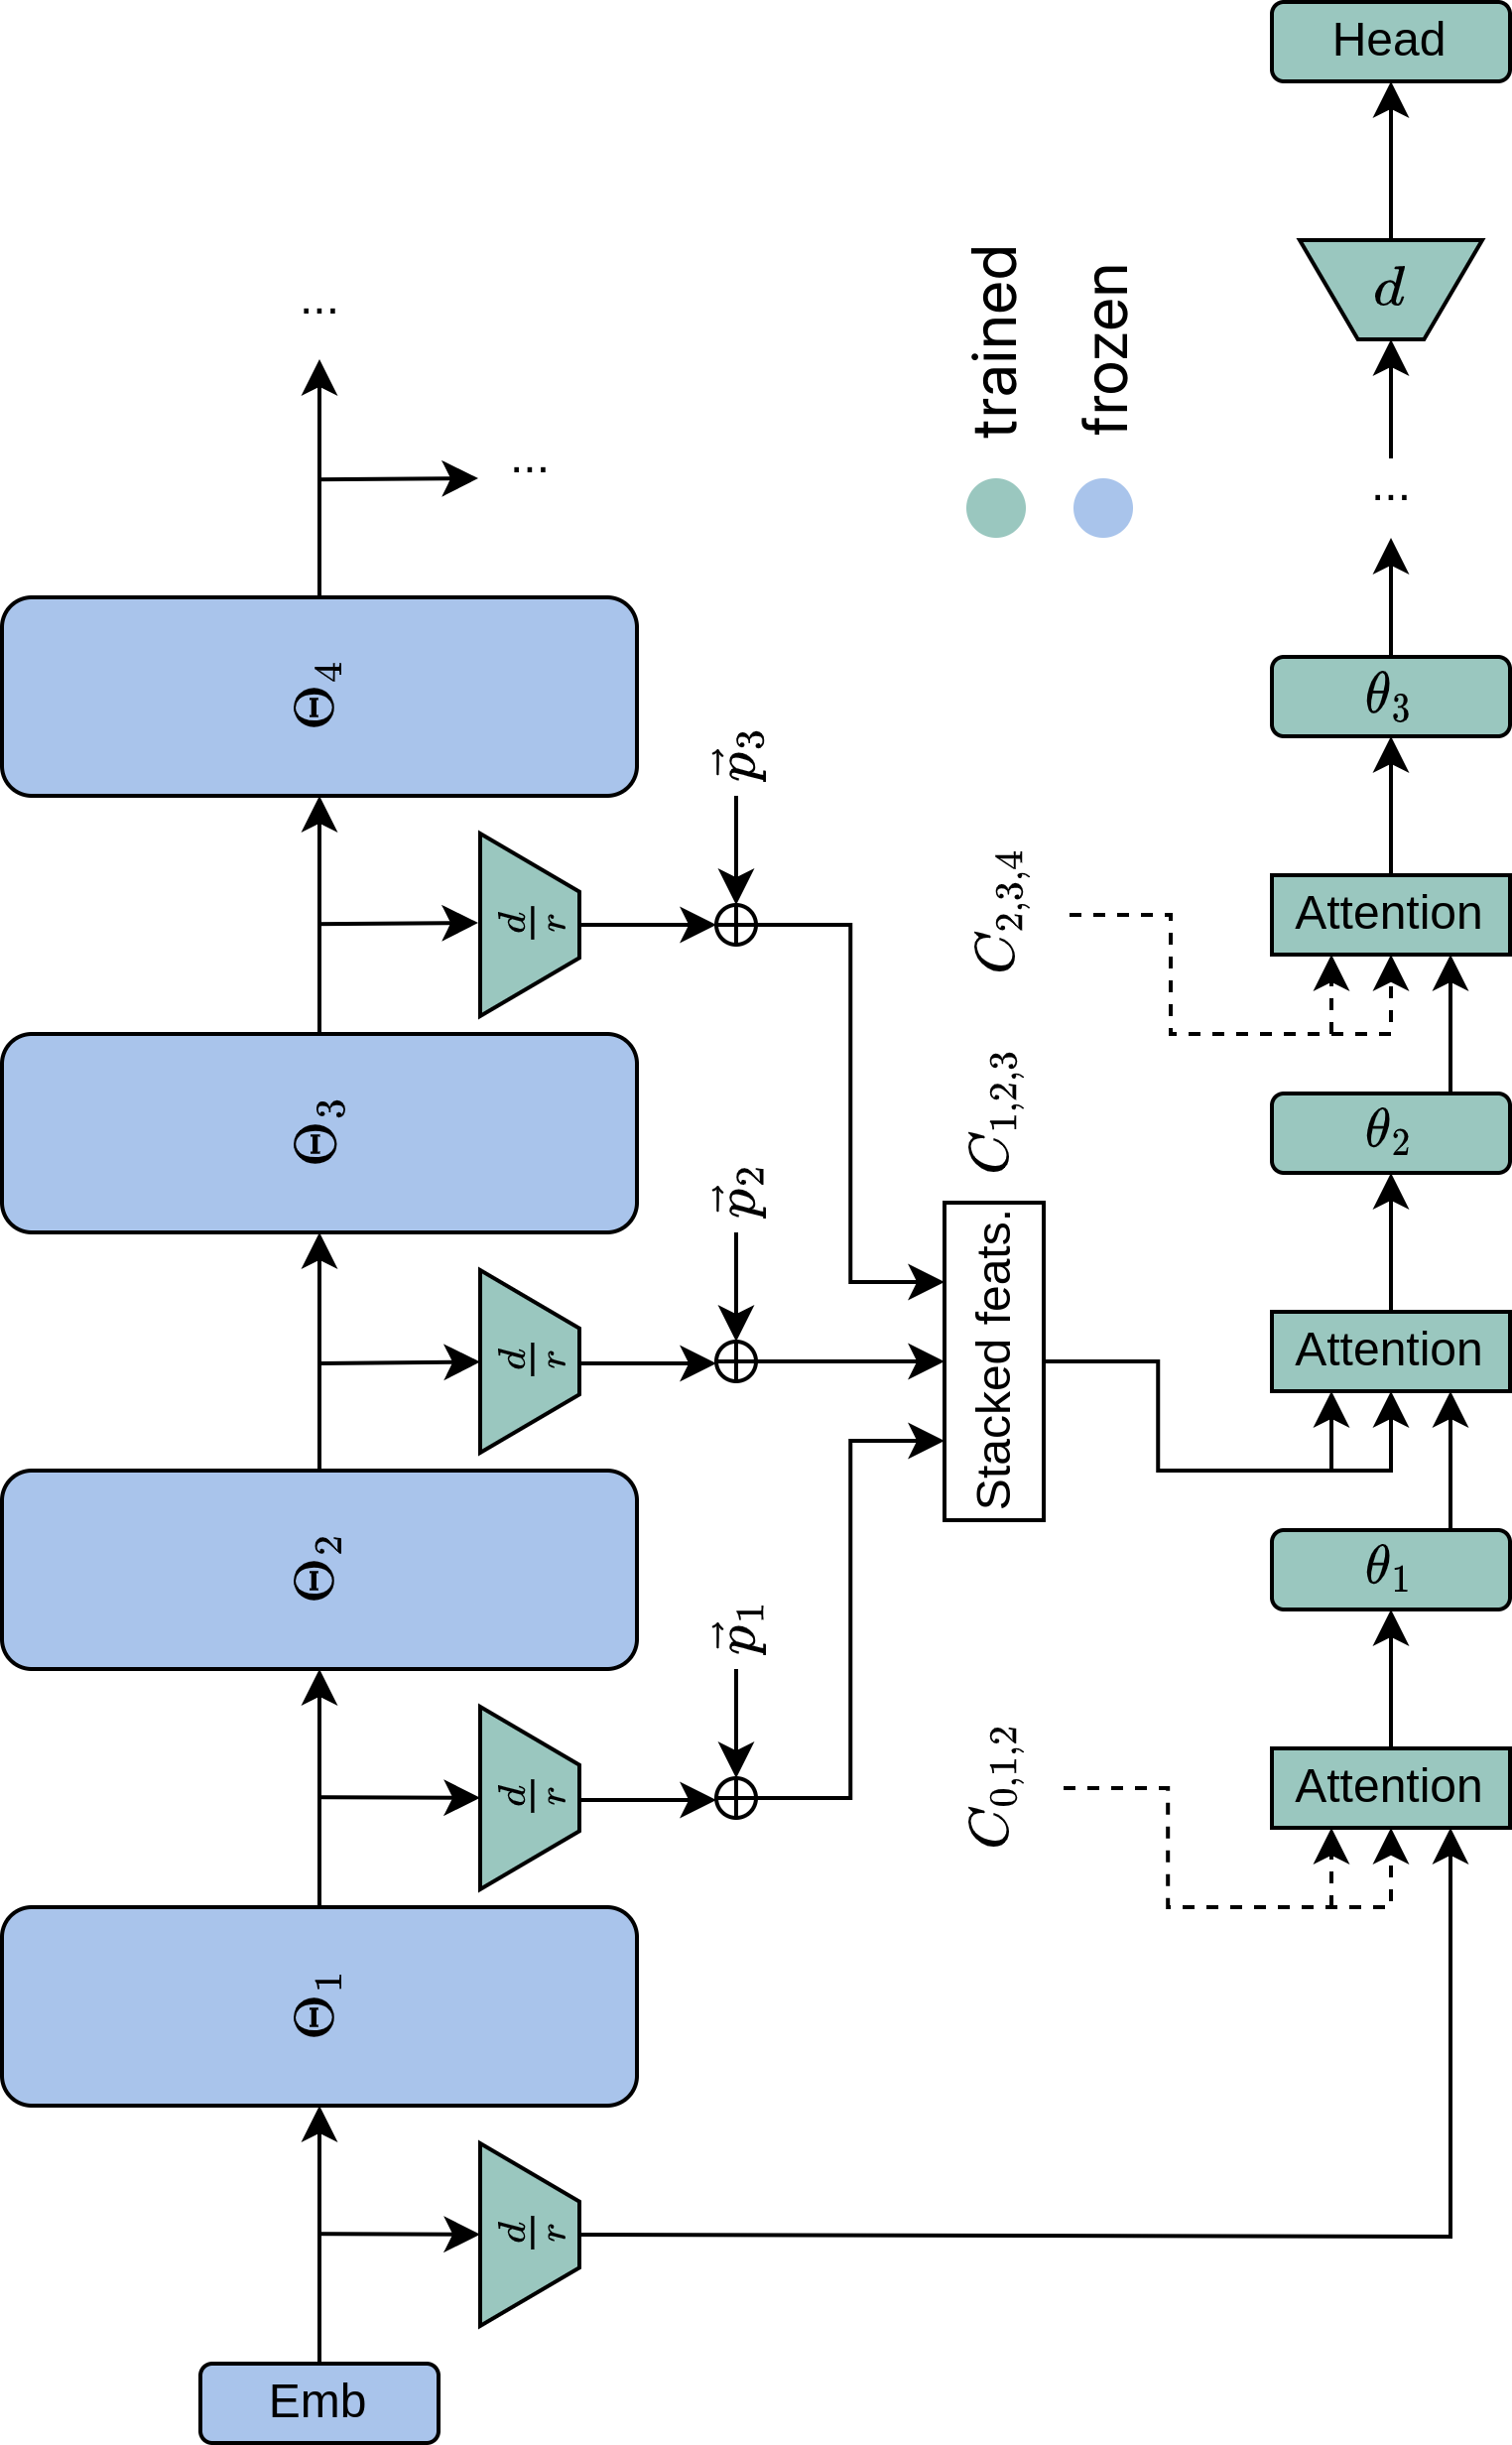
\includegraphics[width=0.4\textwidth, angle=-90]{assets/images/k-LST.png}
    %\includesvg[width=0.5\textwidth, angle=-90]{assets/images/k-LST.svg}
    \caption{This figure shows the k-LST diagram for \(k = 3\). Only the added parameters and head are trained (shown in green), while the backbone remains frozen (shown in blue). We first downsample each feature with a linear projection, before adding the positional encoding and concatenating the features into a single matrix. The features are queried with cross attention by the side network. The backbone's forward pass is completely independent from the side network. The gradients of the trainable parameters can be computed without going through the backbone, resulting in large memory savings.}
    \label{fig:k-LST}
\end{figure*}


\subsubsection{Optimal Hyperparameters}\label{section:lst-parameters}

k-LST has three main hyperparameters: the window size \(k\), the reduction factor \(r\) and the feature dropout probability \(p\). These three parameters provide granular control over the trade-off between memory footprint and performance. A window size of \(k = 9\) showed to be the best performing in our tests. We observed that a higher \(k\) is more susceptible to overfitting. Therefore, for the \(k = 9\) case, we use a feature dropout probability of \(p = 0.2\), while for other experiments we use no dropout. All experiments use a reduction factor \(r = 8\). 9-LST is trained with linear LR decay with warmup. The peak LR is \(\eta = 0.0002\) with a linear decay to \(\text{{2e-6}}\) over \(5\) epochs and a warmup ratio of \(0.12\). All experiments use the AdamW optimizer \cite{DBLP:journals/corr/abs-1711-05101} and the RoBERTa-large \cite{roberta} backbone.


\subsubsection{Benefits for Large Scale Deployments}

The backbone model is completely independent of the side network. This is in contrast to other widely used PEFT methods where the forward pass of the backbone network is directly influenced by the added PEFT parameters. This is a desirable characteristic for large-scale deployment when many different fine-tuned versions of the same backbone model are being served simultaneously. The benefit is derived from the fact that the forward pass of the large backbone model remains constant, regardless of the fine-tuned version. This allows for the batching of requests irrespective of the specific fine-tuned versions. It's a one-way relationship, where the side network has no effect on the output of the backbone model. It simply consumes the intermediate features to produce the final result. As a consequence, there is no need to clone (or dynamically alter) the backbone model. Instead, all requests can pass through the same static backbone model, before the intermediate features are fed into the smaller side networks which can run on smaller compute nodes.

\subsection{MeZO}
Zeroth-order optimization (ZO-SGD \cite{zo-sgd}) estimates gradients using only forward-passes, making it possible to update neural networks without backpropagation. Memory-efficient Zeroth-order Optimizer (MeZO \cite{mezo})  is an adaptation of the classical zeroth-order optimization method, reducing its memory consumption by operating in-place. This results in a method that is able to fine-tune LMs with the same memory footprint as inference. 
%The authors prove that MeZO can successfully optimize LLMs and show its efficiency 

To estimate gradients, MeZO uses Simultaneous Perturbation Stochastic Approximation (SPSA), which requires two forward passes to estimate the gradient. For each forward pass, the parameters of the model are perturbed by different amounts, depending on a random number sampled for each parameter and the perturbation scale, which is a hyperparameter of the model. For loss function $\mathcal{L}$, model parameters $\mathbf{\theta} \in \mathbb{R}^d$ and minibatch $\mathcal{B}$, SPSA estimates gradient as:

\begin{equation}
    \hat{\nabla}\mathcal{L}(\mathbf{\theta}; \mathcal{B}) = 
    \frac{\mathcal{L}(\mathbf{\theta} + \epsilon\mathbf{z}; \mathcal{B}) - \mathcal{L}(\mathbf{\theta} - \epsilon\mathbf{z}; \mathcal{B})}
    {2 \epsilon} \mathbf{z}
\end{equation}

where $\epsilon$ is the perturbation scale and $\mathbf{z} \in \mathbb{R}^d$ is randomly sampled with $\mathbf{z} \sim \mathcal{N}(0, \textbf{\em I}_d)$. 

Using the SPSA estimate for gradients, the model is updated with SGD:

\begin{equation}
    \mathbf{\theta}_{t+1} = \mathbf{\theta}_t - \eta \hat{\nabla} \mathcal{L}(\mathbf{\theta}; \mathcal{B}_t)
\end{equation}

where $\eta$ is the learning rate. 

MeZO's in-place implementation saves additional memory for this approach. For each batch, MeZO samples a random seed and every time a parameter gets updated or perturbed for the gradient estimation, it samples the random value \textbf{z} using this seed. This way, $\mathbf{z} \in \mathbb{R}^d$ does not need to be stored, theoretically reducing memory consumption to the same as inference. In practice, often entire weight matrices are perturbed instead of individual scalars, saving time but costing additional memory as large as the largest weight matrix. 

\subsubsection{Prompt-based Fine-tuning}

Experiments show that prompting is crucial for the ability of MeZO to optimize the network. Thus, MeZO is used under the prompt-based fine-tuning setting described in \cite{prompt}. 

For each example in the dataset, a model is given a prompt as input; this prompt is a template attached to the input sentence and varies depending on the task and dataset. The template contains a mask token and the model is trained to predict the masked word from a set of label words, where each label word is assigned to one label. Classification is then performed using the logits of the label words on the mask token. \Cref{fig:prompt} shows how prompt-based fine-tuning works on the SST-2 dataset. 

\begin{figure}
    \centering
    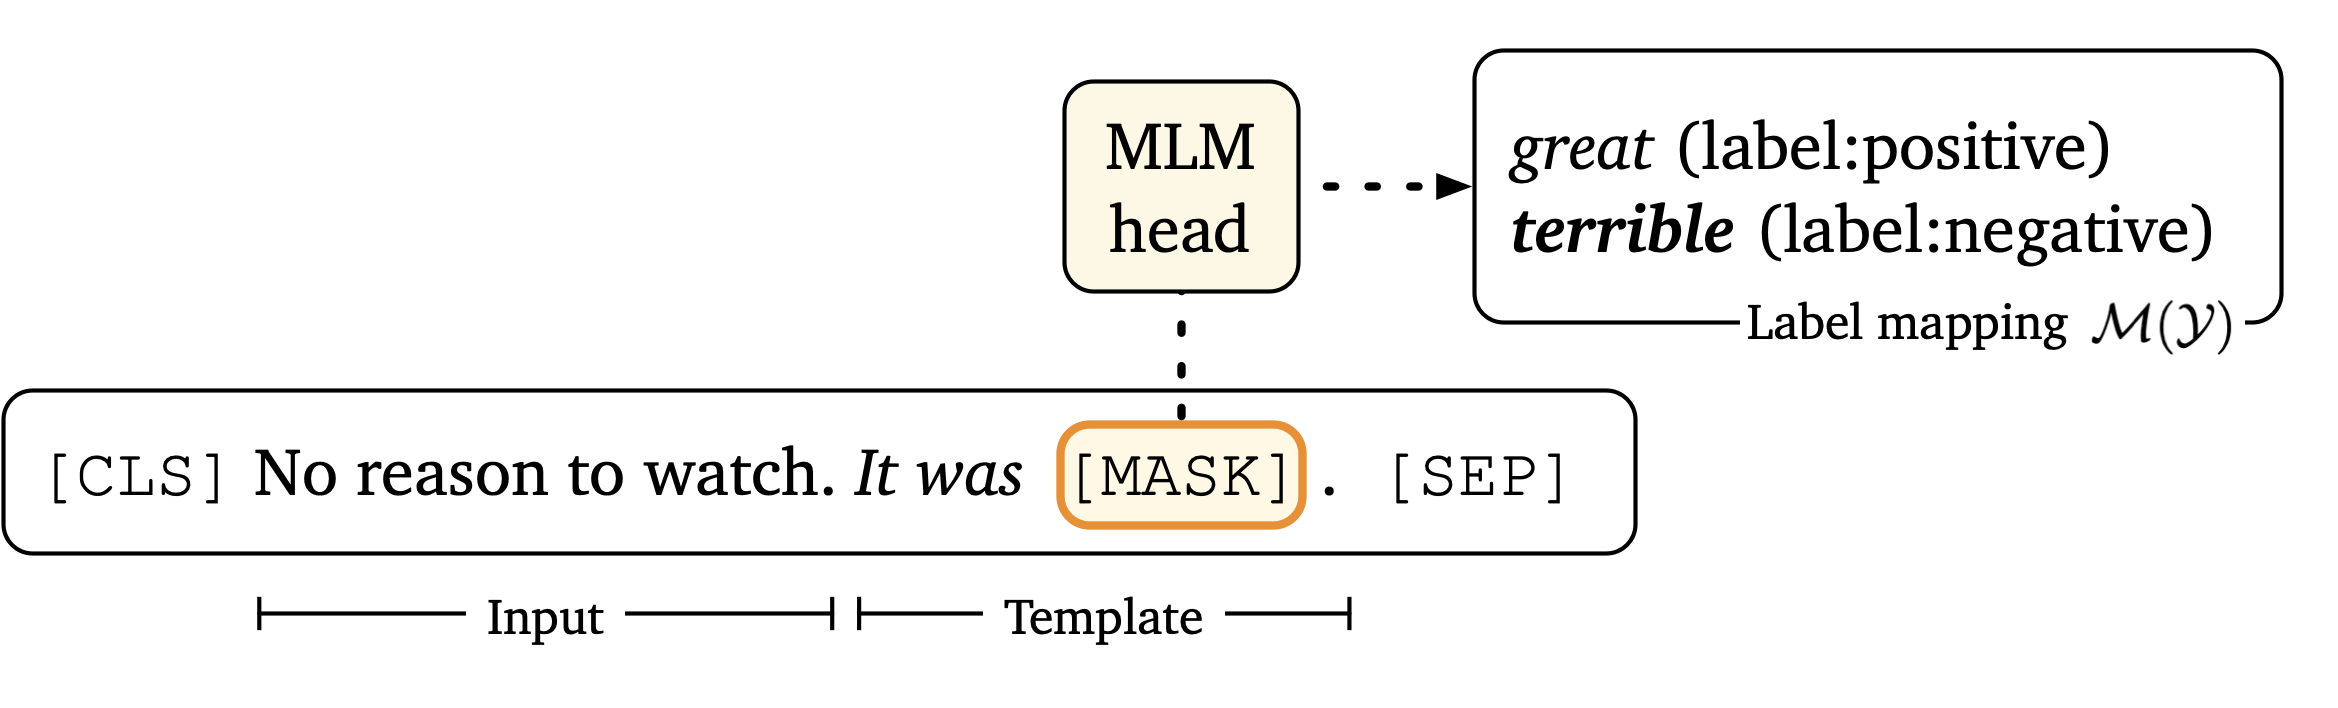
\includegraphics[width=\linewidth]{assets/images/Prompt.png}
    \caption{Prompt-based fine-tuning on SST-2. Adapted from \cite{prompt}. The prompt consists of the input sentence and the template \textit{"It was [MASK]."}. The model is trained to predict the label word \textit{"great"} for positive input sentences and \textit{"terrible"} for negative input sentences.}
    \label{fig:prompt}
\end{figure}


\begin{table*}[htb]
  \caption{Comparison of Different Methods when fine-tuning a RoBERTa-large model on the SST-2 dataset using a batch size of 16. Samples per Second is measured on an RTX 3070 Mobile and computed as the number of all training samples divided by the total time of training.}
  \label{method-comparison}
  \centering
  \begin{tabular}{lcccc}
    \toprule
    Method           & Accuracy & F1    & Memory Usage (MB) & Samples per Second    \\
    \midrule
    Full Fine-Tuning & 96.44    & 96.52 & 8188              & 51.8                  \\
    LoRA             & 96.22    & 96.30 & 4526              & 64.6                  \\
    LST              & 93.23    & 93.33 & 1779              & 73.8                  \\
    Last 3 Layers    & 94.04    & 94.18 & 2117              & 179.6                     \\
    \midrule
    SiVA             & 96.56    & 96.63 & 4529              & 73.3                  \\
    SiVA - key value & 95.76    & 95.86 & 2920              & 106.4                 \\
    \midrule
    5-LST            & 94.04    & 94.04 & 2209              & 60.3                  \\
    9-LST            & 95.07    & 95.18 & 2381              & 52.4                  \\
    %\midrule
    %MeZO    &   91.74   & 91.96     &   1805    &   54.5
    %                \\
    \midrule
    LST + Prompt  & 94.84    & 94.98 & 1803              & 73.8                  \\
    9-LST + Prompt& 95.41    & 95.55 & 2428              & 52.4                  \\
    Last 3 Layers + Prompt & 94.84 & 94.87 & 2122 & 179.6 \\
    \bottomrule
  \end{tabular}
\end{table*}

\section{Results}

\Cref{method-comparison} shows a comparison of our methods and their respective baselines. We evaluate the performance in terms of accuracy and F1-score on the SST-2 dataset, as well
as peak memory usage and training samples per second. For all experiments, we fine-tune a RoBERTa-large model using a batch size of 16. 

Both SiVA and k-LST improve upon their respective baselines (LoRA and LST), while prompts bring improvement irrespective of the PEFT method they are used with. As a result, we present a set of new PEFT methods that cover both the low memory and full fine tuning quality regimes:

\begin{itemize}
    \item SiVA can be used to achieve a balanced reduction in memory usage and computation time when no compromise can be made on model performance.
    \item k-LST can be used to achieve the highest reduction in memory usage with minimal loss of model performance.
    \item Prompting can be used in conjunction with layer freezing or k-LST to further increase fine-tuning performance at no additional cost.
\end{itemize}


\section{Conclusion and Future Work}

\subsection{Conclusion}
In this work, we introduced two new PEFT methods. Our low-rank update method SiVA represents weight matrices in a lower rank using SVD. SiVA converges much faster than the competition (LoRA), keeping the full-fine tuning accuracy and low memory usage.

Our low memory PEFT method, k-LST, presents a generalization of the original LST by extracting backbone features from a k-sized window. The side network queries these features using cross-attention. k-LST converges faster and achieves higher accuracy than LST while keeping a low memory footprint. This presents a significant step in closing the performance gap of memory efficient PEFT methods.

In addition to our new PEFT methods, we used modified prompts during fine-tuning with different PEFT methods and measured an improvement in performance metrics without any downsides. As a result, we recommend SiVA for high-accuracy fine-tuning and k-LST with prompts for low-memory fine-tuning.

\subsection{Future Work}
As future work, we recommend testing larger models with various architectures on more benchmarks to better understand our methods' performance benefits. Additionally, SiVA and k-LST can be combined together or with different PEFT methods to achieve further performance benefits. Both SiVA and k-LST are model agnostic, so testing domains other than NLP and non-transformer models remains a promising direction for future research.

For SiVA specifically, the \(W_r\) matrix could be represented in lower precision for higher efficiency. QLoRA's 4-bit quantization \cite{dettmers2023qlora} could be adapted for use with SiVA in order to produce highly accessible, quantized LLMs with better accuracy.

k-LST remains a fruitful research direction for future research. Further work can be done by experimenting with weight sharing and techniques similar to the original LST's LayerDrop to lower computational and memory costs. Additionally, pretraining the side network jointly with the backbone could further close the performance gap. Pretraining could enable the side network to learn how to use backbone features efficiently in a general context before it is fine-tuned for a specific use case.

For prompting, experimenting with different prompts could prove to be beneficial. In particular, an automatic prompt generation pipeline can be incorporated as in LM-BFF \cite{prompt}.

\printbibliography

\end{document}
